\chapter{IP-core Manager functionalities}
\label{chap1}
\section{Enabling the right IP}
The first and basic task for this core manager is to enable the connection between the CPU and the selected core. More in particular this means exchanging the data in the required time as described in the protocol. The CPU can talk to one and only one core, therefore the core manager will disregard other cores whether they finished or not their task.
We know that the CPU writes at $ row_{0} $ what it wants to do. Here we can read the physical address of the chosen IP core.
If we know that the $ 1^{st} $ core is selected, than the IP manager has to enable the $ 1^{st} $ core (i.e. $port_{0}  $) and disable all the other ones, thus having the following signal:\\
\begin{center}
	$ enable_0='1' $\\
$ enable_1='0' $\\
$ enable_2='0' $\\
$  \vdots $\\
$ enable_{n-1}='0' $
\end{center}
\bigskip
We can put all these signal together as if they were an array.\\
\bigskip
To make this kind of operation, a conversion is required.\\
We can clearly see that only one bit is at $ '1' $, while the others are at $ '0' $, this is due because the CPU can talk at most to only one IP-core.\\
The feature of having at most one bit at '1' is the well known \textit{one hot encoding}.\\
We implicitly implemented a "kind" of $ bynary $ to \textit{one hot encoding} converter.

At $ row_0 $ we read the physical address, and we raise the right enable signal, keeping the other ones at \textit{'0'}.\\
Figure \ref{fig:en_IP} shows this functionality.\\
\bigskip
A small adjustment has been done, since the physical address \textit{0} is reserved to the IP manager, whilst the  \textit{IP core 0 } has as physical address \textit{1}.\\
\bigskip
This component is active during the rising edge of the clock and when the CPU wants to start a transaction.
\begin{figure}[h!]
	\centering	
	\includegraphics[width=0.7\textwidth]{imm/ip_func/enable_ip.png}  
	\caption{Enabling the right IP core} 
	\label{fig:en_IP}
\end{figure}
\bigskip
This is the VHDL code that perform this task
\begin{lstlisting}
-- Begin ( or continue ) transaction:
if row_0(BE_POS) = '1' then											
enable_IPs(conv_integer(row_0(IPADD_POS downto 0))-1) <= '1';
data_in  <= data_in_IPs(conv_integer(row_0(IPADD_POS downto 0))-1);
data_out_IPs(conv_integer(row_0(IPADD_POS downto 0))-1) <= data_out ;
add <= add_IPs(conv_integer(row_0(IPADD_POS downto 0))-1);
W_enable <= W_enable_IPs(conv_integer(row_0(IPADD_POS downto 0))-1);
R_enable  <= R_enable_IPs(conv_integer(row_0(IPADD_POS downto 0))-1);
generic_en <= generic_en_IPs(conv_integer(row_0(IPADD_POS downto 0))-1);																		

\end{lstlisting}
\clearpage
\section{Connecting the signals}
The IP core Manager has the duty to make possible the exchanging of data between the CPU (buffer) and the selected IP core, in both direction i.e. from CPU to the IP core and from the IP core to CPU.
In order to select the right input among the \textit{N} ones og the IP cores, we can just look at $ row_0 $, bits $ [11:0] $, because here there is the physical address of the selected core.
\bigskip
%\begin{figure}[h!]
%	\centering	
%	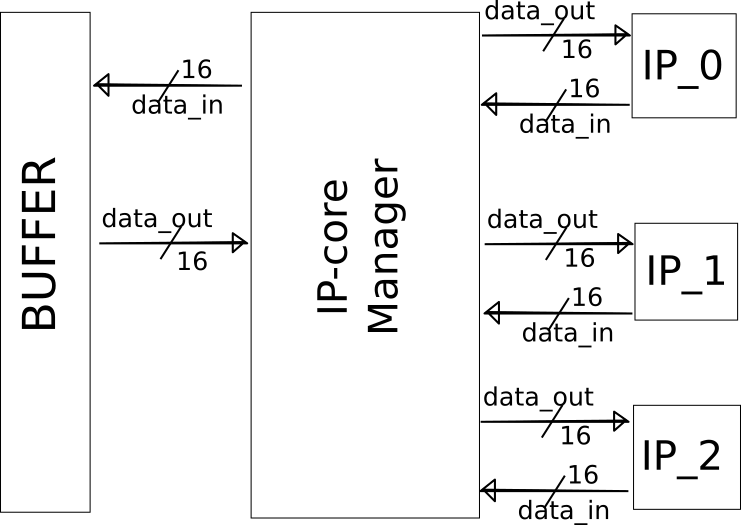
\includegraphics[width=0.9\textwidth]{imm/ip_func/x_switch.png}  
%	\caption{Cross switch} 
%	\label{fig:x_switch}
%\end{figure}

\begin{figure}[h!]
	\centering	
	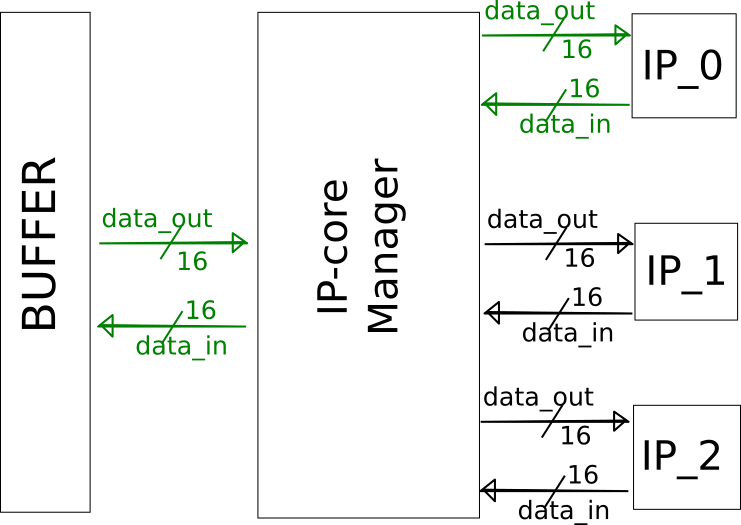
\includegraphics[width=0.85\textwidth]{imm/ip_func/x_switch22.png}  
	\caption{connecting the signal with $ IP0 $, supposing $ row_0 $ ask for the first IP core} 
	\label{fig:x_switch1}
\end{figure}
\bigskip

\begin{figure}[h!]
	\centering	
	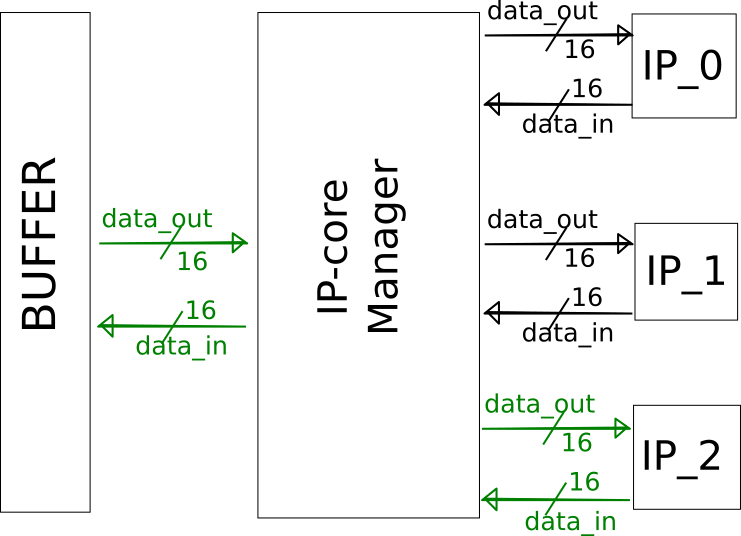
\includegraphics[width=0.85\textwidth]{imm/ip_func/x_switch33.png}  
	\caption{connecting the signal with $ IP2 $ supposing $ row_0 $ ask for the third IP core} 
	\label{fig:x_switch2}
\end{figure}

\clearpage
\section{Interrupt Handler}
The IP-core manager has to manage the case when a single or multiple core raise an interrupt request. 
However since the architecture is a master (CPU) slave (FPGA) architecture, the IP manager must guarantee that an interrupt request from one or more of IPs do not interrupt a transaction started by the master. In order words, the interrupt handler will be active at the end of a transaction.\\
In the case when multiple core raise the interrupt, the IP core manager will give priority to the core with the most priority level which is connected to the lowest port i.e. $ port_0 $.\\
In order to do so, we collect all the $ interrupt_x $ signals of the cores into an array. Than we search for the LSB at \textit{'1'}. Finally we convert the position of this bit into the physical address of the core requesting the interrupt.\\

\begin{figure}[h!]
	\centering	
	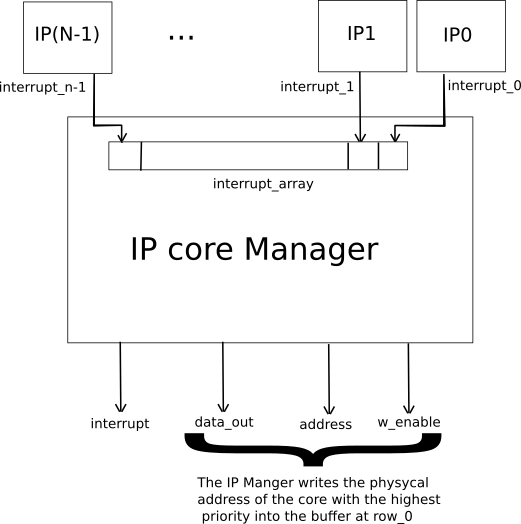
\includegraphics[width=0.85\textwidth]{imm/ip_func/interrupt.png}  
	\caption{Interrupt Handler} 
	\label{interrupt}
\end{figure}
The work of the IP Manager is first to check if there is any interrupt, this can be done by comparing the value of the interrupt vector. If the value is zero, that means that nobody raised the interrupt.\\
Otherwise it has to find the core with the highest priotiy.\\
In order to do so, it can iterate \textit{N} times, i.e. from $ i=N-1 $ to $ i=0 $. In this loop it checks the bit in \textit{Interrupt\_array(i)}, if it is $ '1' $, then the variable $ i $ is the physical address of the IP core requesting an interrupt. However, we keep the loop, because it is possible to have an IPcore with an higher priority.
\begin{figure}[h!]
	\centering	
	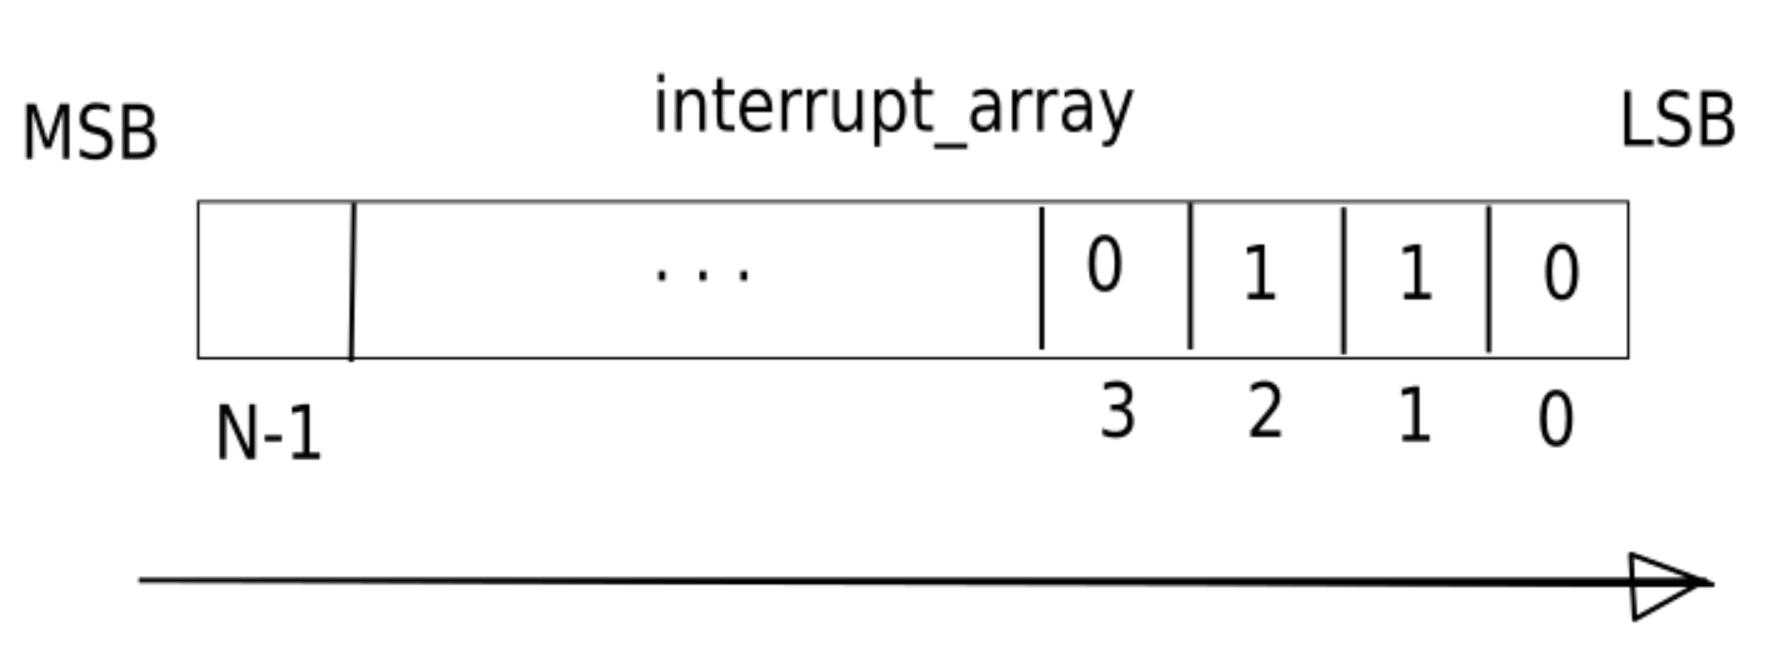
\includegraphics[width=0.85\textwidth]{imm/ip_func/int_vector.png}  
	\caption{A possible interrupt vector} 
	\label{int_vector}
\end{figure}\\
For instance, let's take the interrupt vector shown in fig. \ref{int_vector}.\\
When iterating with $ i=2 $, we wants to send the address of the third core, but when we decrease the counter $ i=1 $, we have to update this address. When $ i=0 $ we leave everything unchanged.
 